\begin{longtable} { | c | p{12cm} | c | } 
\hline
	ID 	&	Issues	&		 Es. hours \\\hline
	5	&	Copying Sequences	&	16 hours	\\\hline
	24	& 	Delete Sequences	&	2 hours \\\hline
	59  	&	Implement delete/copy with database	&	1 hour \\\hline
\caption{Issue ID 5, 24 and 59}
\label{tab:spr4_copyingsequences}
\end{longtable}

From the report last semester, it was stated that future work could include a copy feature to copy sequences from one child to another. This would however not have made sense to implement before having the database ready, and was thus postponed to the last sprint. The feature was implemented as a new button in the overview. When clicking the button, a pop-up window would appear where the user can press the sequences to copy. Pressing one will then move from a grid on the left (holding all sequences) to a grid on the right part of the screen. Pressing the "Copy and send to" button below will then display a GComponent, displaying all children belonging to that guardian, enabling the user to pick N children to copy M sequences to at the same time. This is illustrated in figure \ref{fig:copyDialog} and figure \ref{fig:profilesList}.

\begin{figure} [ht!]
\centering
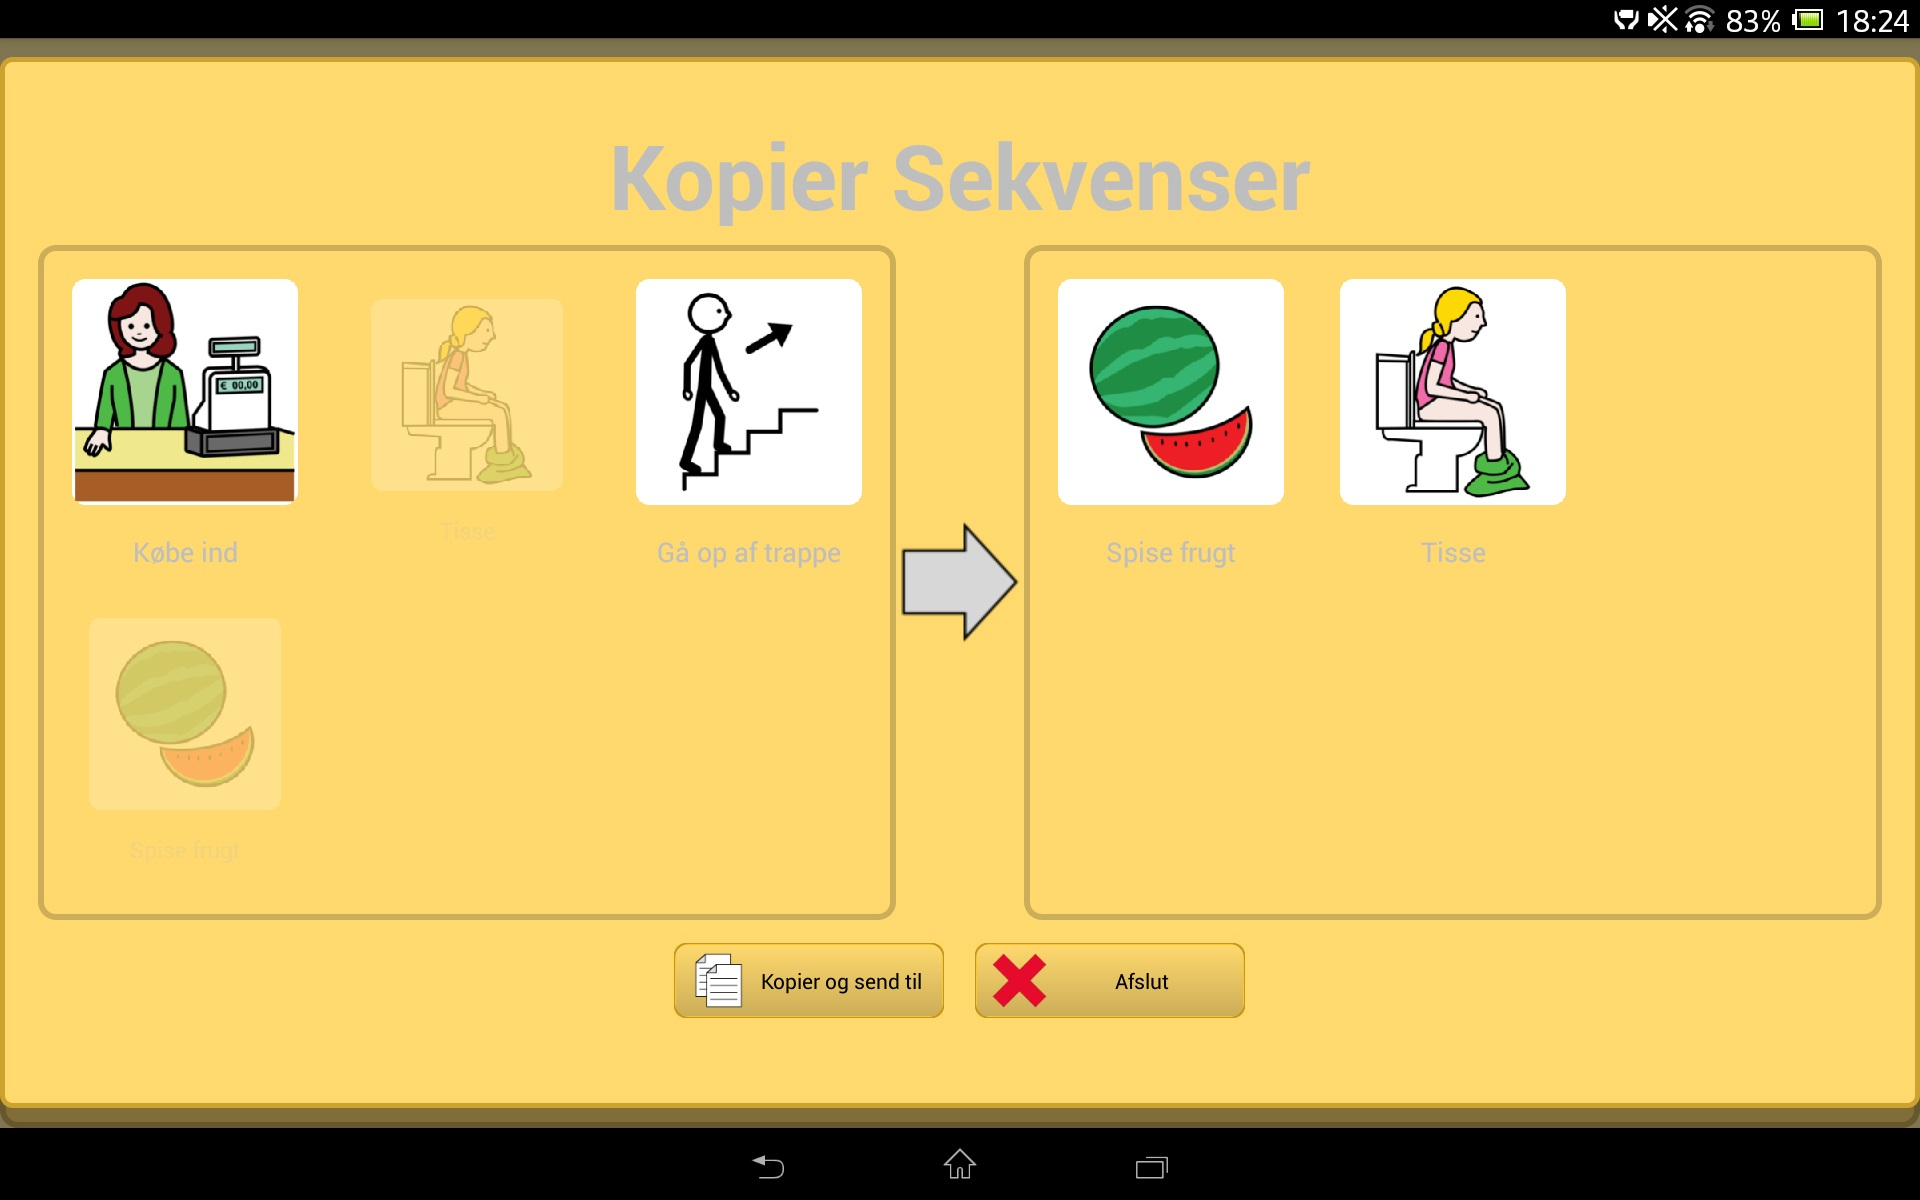
\includegraphics[width=0.6\textwidth]{Pics/Sprint4/copyPasteDialog/copy}
\caption{An example of a user trying to copy 2 different sequences}
\label{fig:copyDialog}
\end{figure}
\begin{figure} [ht!]
\centering
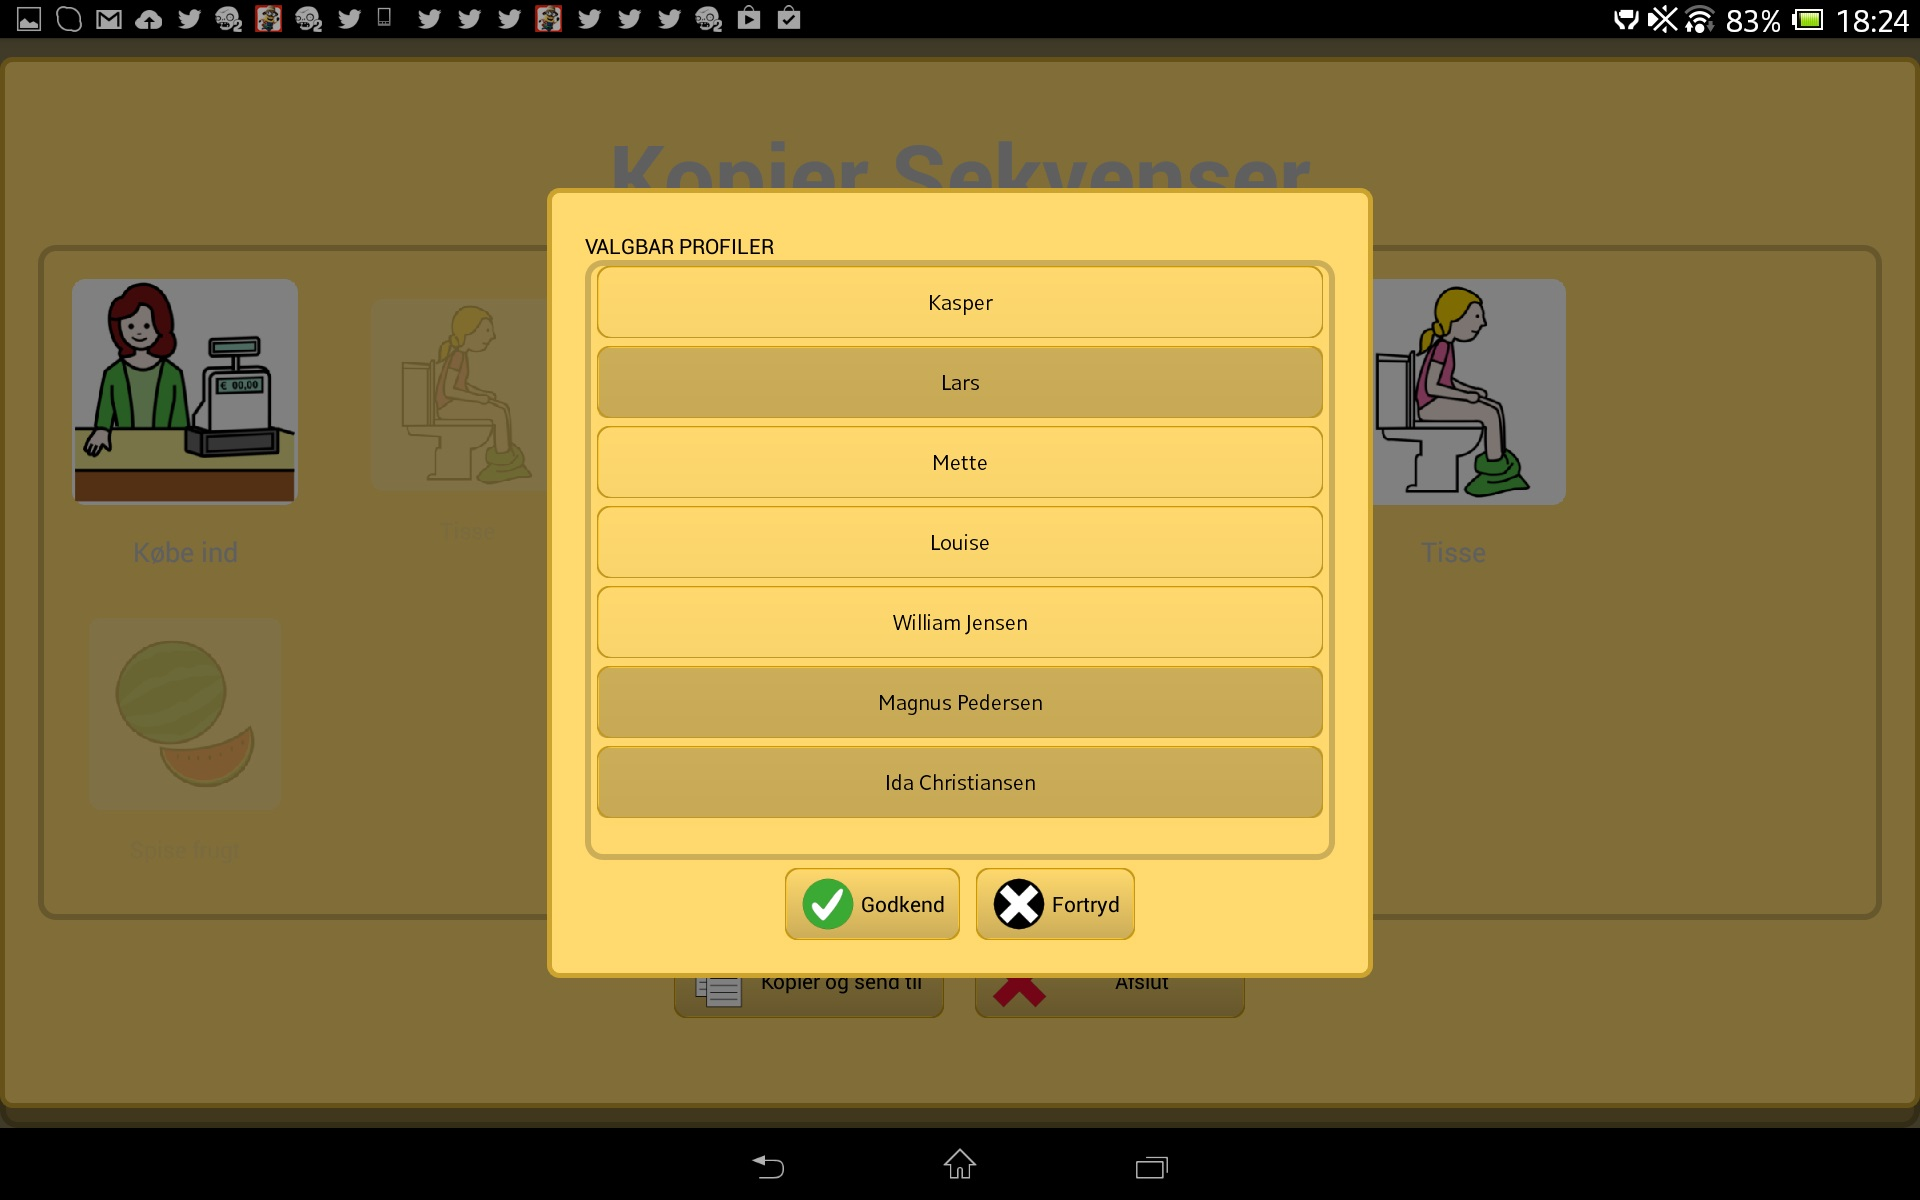
\includegraphics[width=0.6\textwidth]{Pics/Sprint4/copyPasteDialog/profilelist}
\caption{An example of a user trying to copy sequences to 3 different children at the same time}
\label{fig:profilesList}
\end{figure}

At the beginning of the semester it was actually possible to delete sequences, although these sequences were not part of the database. It was however very easy to accidentally delete sequences as a delete button was placed on every sequence when logged in as a guardian. There was no confirmation of deletion either. Therefore it was chosen to implement the delete functionality similar to the copy feature. A button was added which would create a pop-up window. Here, the user can press the sequences to delete, and press the delete button to perform the action. This means the user would have to mis-press two times to accidentally delete a sequence.

The reason the pop-up window was designed with the dual-grid was because a drag-and-drop functionality was intended. Unfortunately there was a major look-over in that dragging already was used for scrolling in the list of sequences, making it impossible to have both drag functionalities. Due to time constraints, the view was not altered, but was implemented to register a user press instead. If time had allowed it, a better solution could have been to have one big grid where one could add checkmarks to the sequences one wanted to delete or copy. This unexpected issue also meant that these issues went a few hours over the expected estimates.

After closing the issue it was discovered that the implementation uses an excessive amount of memory. This means that working with over 25-30 sequences at a time can crash the application with an \ct{OutOfMemoryException}. As this task was only closed in sprint 4 however, there was not time for a redesign.
\clearpage